\chapter{L'aboutissement du projet}
\label{chap:aboutissement}

Le développement du site achevé permet alors de voir avec un peu plus de recul ce qui a concrètement été réalisé, rajouté ou abandonné. Tout cela permet également une comparaison avec les objectifs initiaux du projet donnés en grande partie par la maquette du site.

\section{Les pages de formalités}
\label{sec:pages-formalites}

% home page screenshot
\begin{figure}[h]
    \centering
    
\includegraphics[width=\textwidth]{assets/pictures/home-page.png}
    \caption{Page d'accueil du site de l'\ofni}
    \label{fig:home-page}
\end{figure}

Le site contient un certain nombre de pages de formalités, qui sont des pages statiques pour la plupart. On y trouve notamment l'accueil du site, que l'on peut voir \figureref{fig:home-page}, la page de présentation de l'association, celle d'adhésion ainsi que celle des mentions légales. Certaines de ces pages sont présentent des informations qu'il est, juridiquement, obligatoire de faire apparaître sur un site web. C'est le cas des mentions légales, qui sont des informations sur l'association, son siège social, son numéro de téléphone, son adresse \langue{e-mail}, son numéro de \logo{SIRET}, etc.

Il est tout de même possible de trouver un petit peu de dynamisme sur certaines pages, notamment la page d'accueil qui contient des petits \langue{teasers} sur les activités à venir de l'association, ou encore des actualités.

\section{Le jeu \game}
\label{sec:jeu}

% game screenshot
\begin{figure}[h]
    \centering
    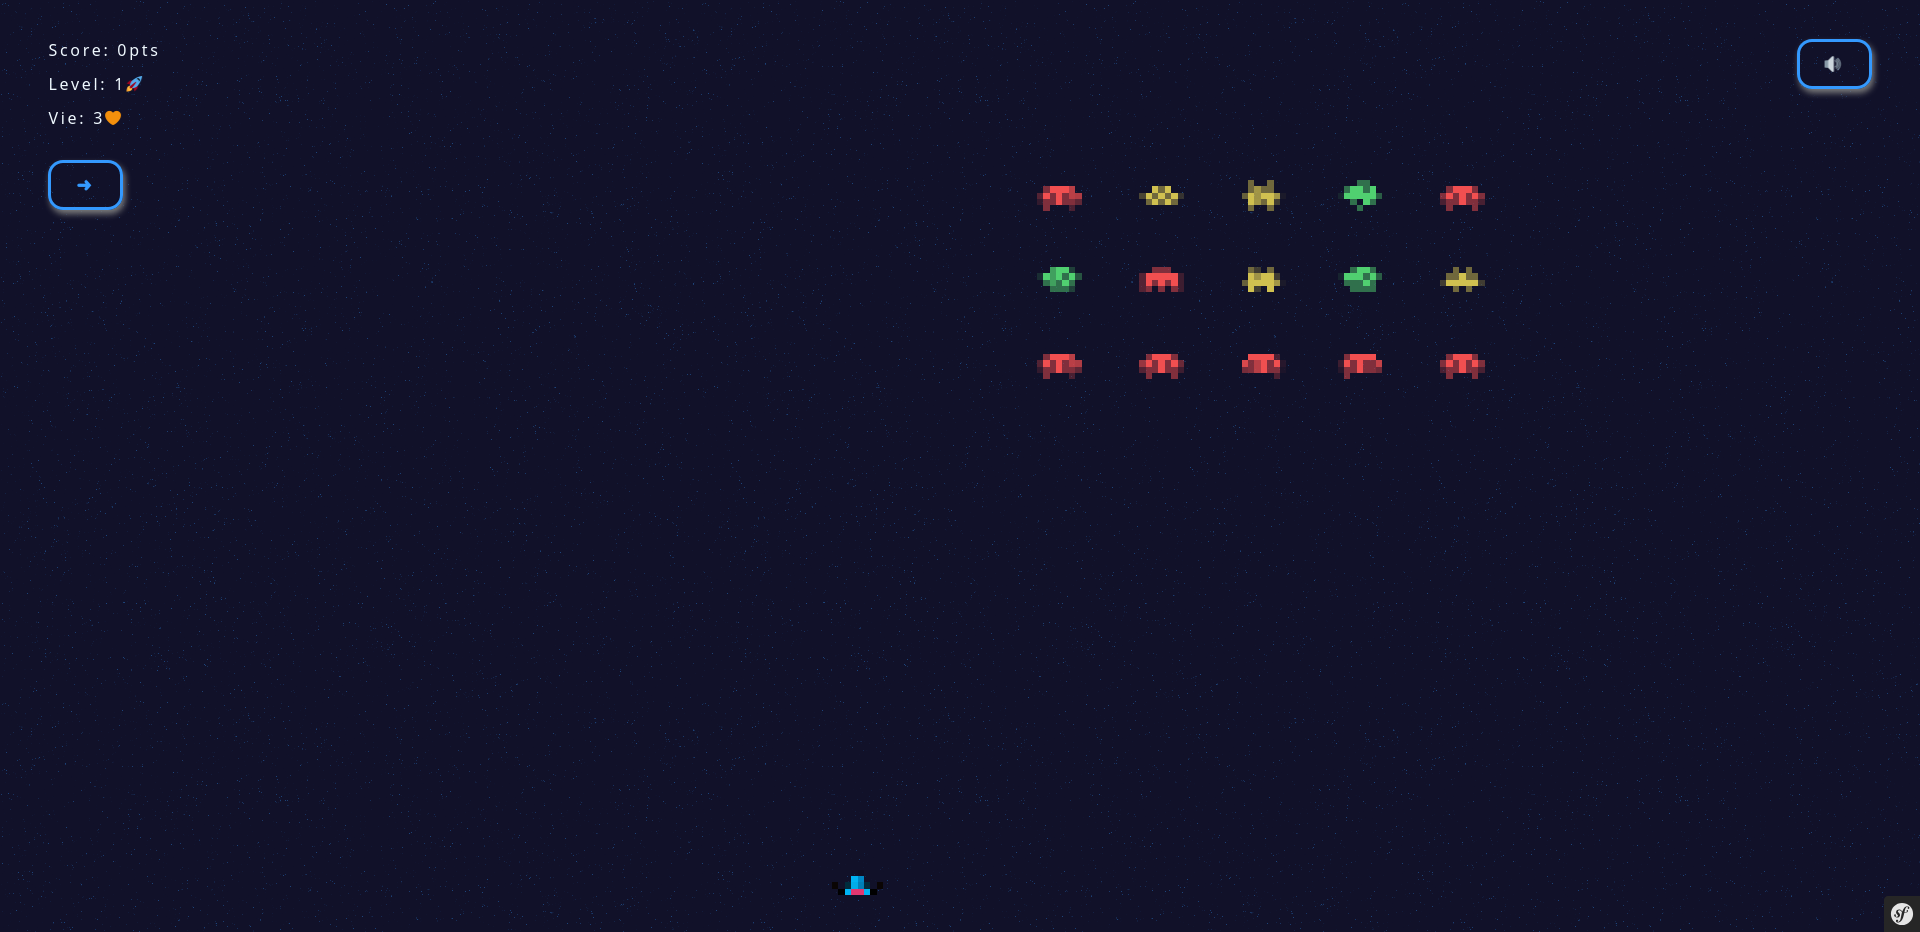
\includegraphics[width=\textwidth]{assets/pictures/game.png}
    \caption{Vue du jeu \game}
    \label{fig:game}
\end{figure}

Peu avant le début de la phase de développement, il fut décider d'ajouter un petit jeu vidéo au site avec un afficage du meilleur joueur pour rendre la visite du site plus attractive. Le jeu \game\ est un jeu de type \citer{Space Invaders} où le joueur doit tirer sur des vaisseaux ennemis pour marquer des points. Le jeu est jouable directement depuis le site, sans avoir besoin de télécharger quoi que ce soit. On peut voir une capture d'écran du jeu \game\ en \figureref{fig:game}.

\section{La connexion et l'inscription aux événements}
\label{sec:connexion-inscription}

Ces actualités et événements de l'\ofni\ constitue la partie centrale du site. Tout cela commence évidemment par un page de connexion, ou de création de compte si l'utilisateur n'en a pas encore. Une fois connecté, l'utilisateur peut alors s'inscrire à des événements.

Comme vu dans la section \ref{subsec:generation-formulaire}, les formulaires d'inscription aux événements sont générés automatiquement à partir des informations de la base de données. Cela permet de ne pas avoir à modifier le code du site à chaque nouvel événement ou bien de réutiliser un même formulaire pour plusieurs éditions.
\bigskip

Lorsque l'administrateur décide de créer un nouveau formulaire, il va en réalité définir ce qui, dans la terminologie du présent site, s'appelle un \formwidget. Il existe trois types de \formwidget\ différents~:
\begin{description}
    \item[Natif] Qui correspond à un champ simple, comme par exemple un texte, une date, ou encore une case à cocher. Ils sont définis par défaut dans le site et ne peuvent pas être modifiés ou ajoutés par l'administrateur. Ils sont les briques fondamentales pour la construction d'autres \formwidget\ plus avancés.
    \item[Composite] Un ensemble de \formwidget\ les uns à la suite des autres. Par exemple, un \formwidget\ composite pourrait être un \formwidget\ natif de type text, suivi d'un \formwidget\ natif de type date, puis d'un autre \formwidget\ composite défini en amont. Ils sont définis par l'administrateur et peuvent être réutilisés dans d'autres \formwidget.
    \item[Liste] Un ensemble de taille indéfinie de \formwidget\ de même type, mais qui peuvent être répétés autant de fois que nécessaire. Par exemple, un \formwidget\ liste pourrait être un \formwidget\ composite décrivant un membre d'une équipe ; l'utilisateur peut alors, lors de son inscription, en remplir autant de fois qu'il ne le faut pour que tous les membres du groupe soient enregistrés. Ils sont définis par l'administrateur et peuvent être réutilisés dans d'autres \formwidget.
\end{description}

Lorsque l'utilisateur s'inscrit à un événement, le formulaire, correspondant à un \formwidget, est alors généré dynamiquement. Il est alors possible de définir des formulaires très complexes, avec des champs de différents types, des champs répétables, etc.
